Phasellus rutrum leo a ornare bibendum. Nam lacus mi, cursus eget cursus non, sodales vel magna. Etiam tristique nisl sed nulla efficitur, at facilisis dui cursus. Vestibulum at feugiat nulla. Nullam feugiat placerat augue vitae faucibus Figura \ref{maxwell}. Nullam feugiat ligula eu massa bibendum imperdiet. Quisque semper ligula erat. Morbi fringilla elit enim, at dictum quam dignissim eu. Sed ac pulvinar felis, quis posuere augue. Maecenas condimentum mollis enim. Mauris elementum maximus ultricies.

\begin{defi}
Cras cursus, urna et tincidunt varius, elit ligula finibus metus, non laoreet lorem odio vel nibh. Pellentesque pulvinar purus a lacus placerat, a molestie lorem tincidunt. Proin porttitor purus mattis fringilla mollis. Nulla vitae turpis sed urna efficitur egestas ac at nulla.
\end{defi}

\begin{figure}[!htb]
    \centering
    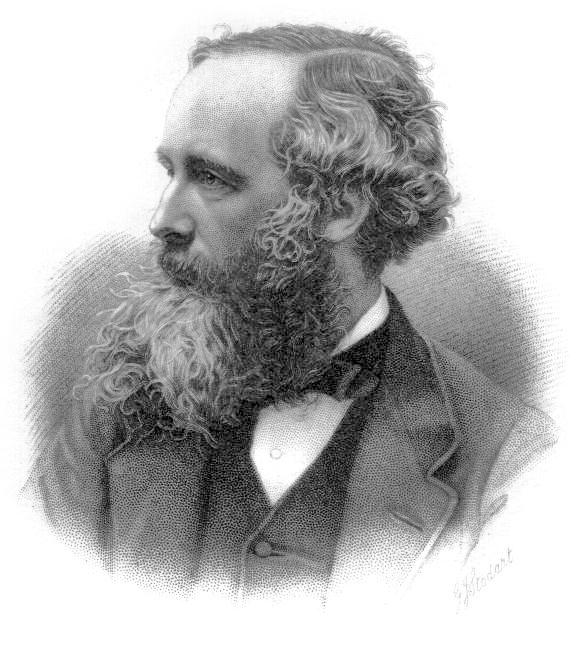
\includegraphics[scale=0.7]{James_Clerk_Maxwell_big.jpg}
    \caption{Maxwell}
    \label{maxwell}
\end{figure}

Etiam quis enim neque. Aenean vulputate et lacus id placerat. Praesent ac nisl at ante condimentum posuere. Vivamus at sagittis mauris. Fusce eget quam elit. Nunc dignissim pharetra dapibus. Mauris id placerat libero, vel molestie sapien.

\begin{description}
    \item[Lei de Gauss] 
                    $$\divfield{E} = \frac{\rho}{\epsilon_{0}}$$
    \item[Lei de Gauss do Magnetismo]
                    $$ \divfield{B} = 0 $$
                    
    \item[Lei de Faraday para Indução]
                    $$\curlfield{E} = -\frac{\partial \textbf{B}}{\partial t}$$
    \item[Lei Circular de Ampère]
                    $$\curlfield{B} = \mu_{0} \left( \textbf{J} + \epsilon_0 \frac{\partial \textbf{E}}{\partial t} \right)$$
\end{description}